\documentclass[11pt,a4paper]{article}
\usepackage{a4wide}
\usepackage{amstext}
\usepackage{pdfpages}
%%\pagestyle{empty}

\begin{document}

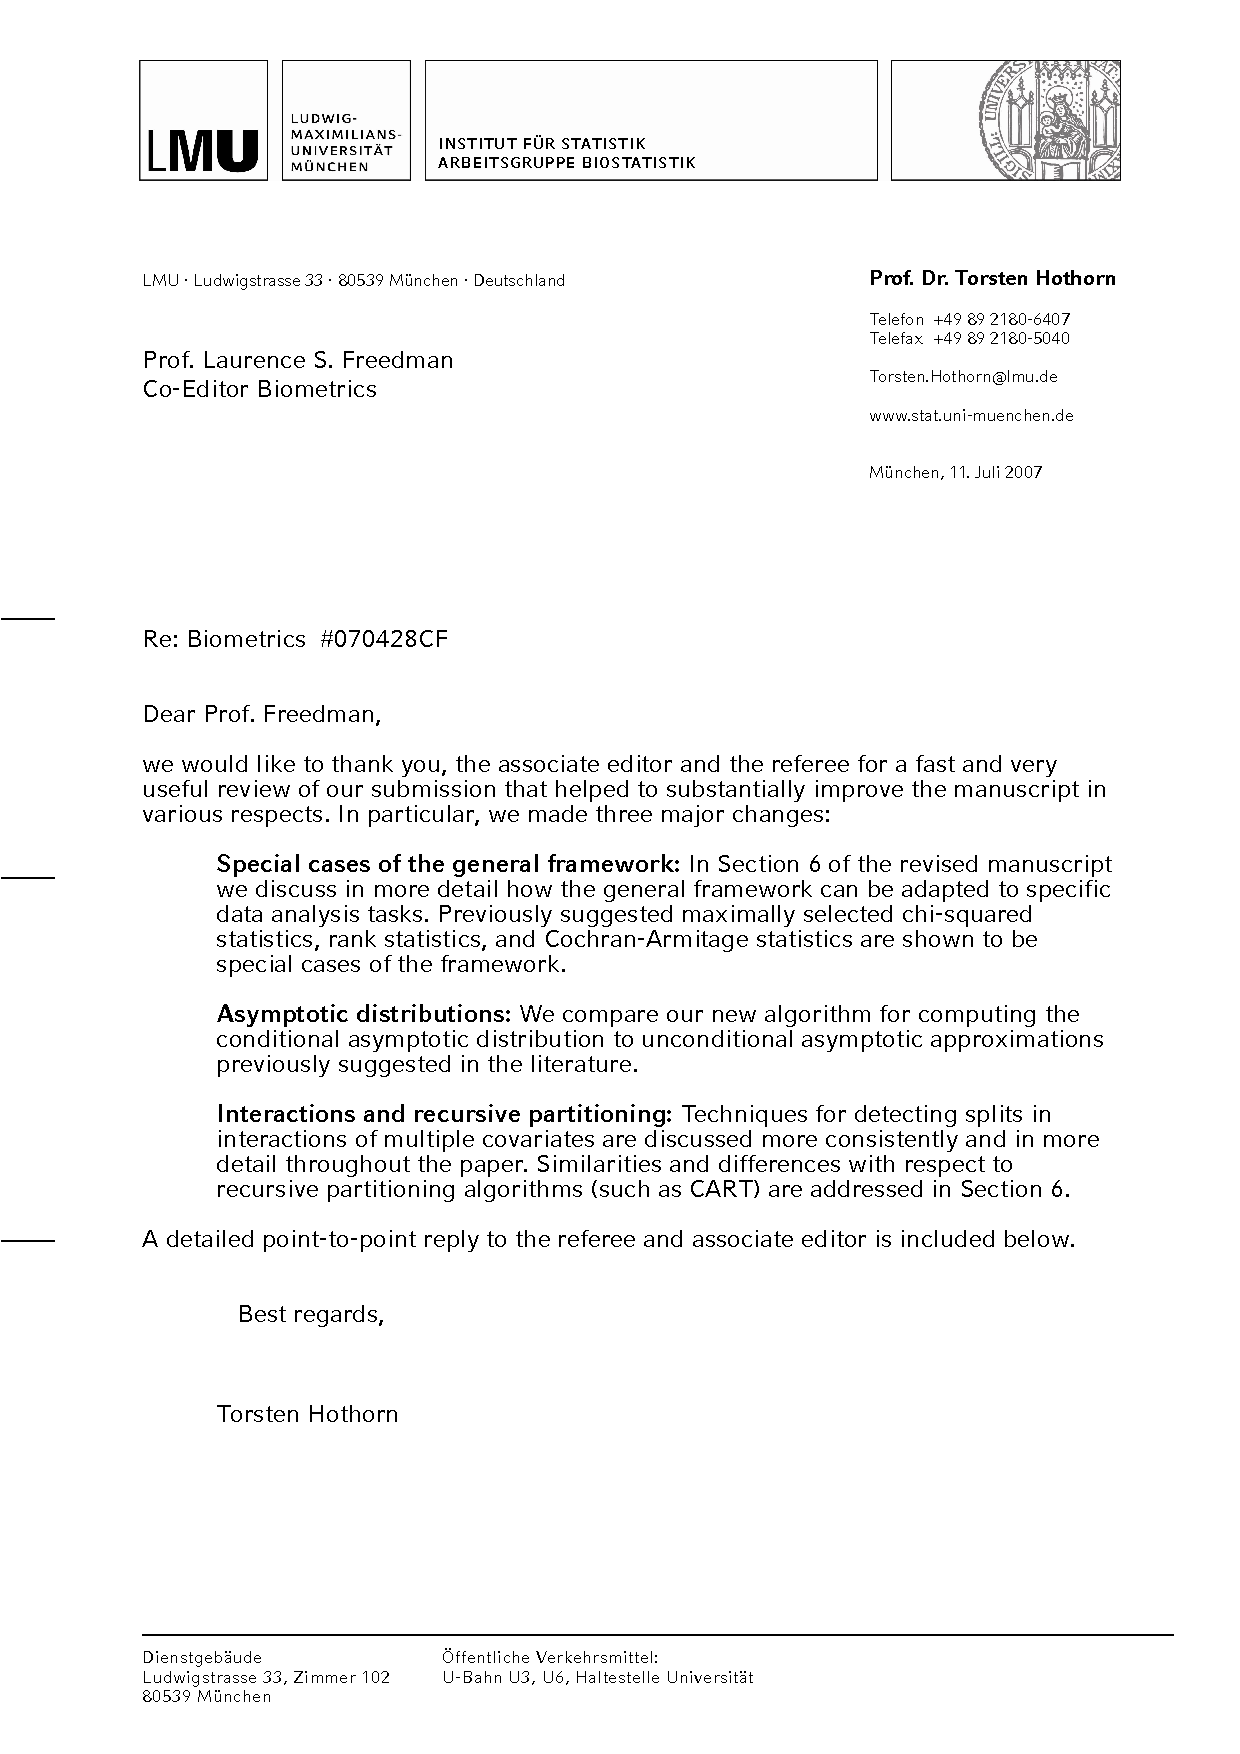
\includepdf[pages=1-]{letter.pdf}

\begin{center}
\textbf{\large Point-to-Point Answers to Manuscript \#070428CF \\
Generalized Maximally Selected Statistics} \\
by Torsten Hothorn and Achim Zeileis
\end{center}

\vspace*{1cm}

\textbf{\large Referee}

General comments:

\begin{itemize}

  \item \textit{The authors claim that most published results on maximally selected
        statistics are special cases of their generalized framework. This sounds very
	attractive, but this affirmation lacks a few explanations/proofs. The
        connections/similarities/equivalences to the other asymptotic approaches
        proposed in previous literature should be outlined/proven in more detail. In
        particular, the present approach is conditional, while most of the previous
        methods are not conditional.}
	
	In Section~6, we show now in more detail how previously established statistics
	are special cases of the generalized framework. Furthermore, we point out 
	more clearly (in Section~5) what the differences between different asymptotic approximations
	for the distribution of the test statistics are.
	
  \item \textit{A simple search in Google Scholar yields other articles: Hothorn and
        Lausen (2003, CSDA), Halpern (1999, Biometrics), Schlittgen (1999, Biom J),
	Burr (2001, Statistics in Medicine), Boulesteix and Strobl (2007),
	Lingyun (1997, JSPI). How do these papers fit into the framework presented here?
	Since the authors' aim is to ``generalize'' maximally selected statistics, as
	many special cases as possible should be enclosed.}
	
        Hothorn \& Lausen (2003) investigate the exact distribution of maximally
        selected rank statistics (now cited in new Section~6). Schlittgen (1999)
        proposes an asymptotic approximation that was assessed in Hothorn \& Lausen (2003)
	and found to be problematic. 

        Halpern (1999) suggests to minimize $p$-values instead of maximizing 
        statistics which is equivalent to other approaches discussed in the paper 
        as long as the asymptotic distribution is used (an exact version is suggested 
        by Halpern in addition).
        Boulesteix and Strobl (2007) propose another exact algorithm for maximally
        $\chi^2$ statistics, the reference has been added.
        Burr (2001) focuses on sums of standard normal distributed statistics
        to detect clusters in a general multiple testing framework that differs
	from the covariate-based approach considered here.
	
  \item \textit{A discussion of the asymptotic approximation's quality would be appreciated.
        What is the behavior compared to other asymptotic approximations already
        proposed in the literature?}
	
	We discuss various asymptotic approximations in Section~5, both for fixed $p$
	and increasing $p$, and show that our new algorithm approximates the exact
	conditional null distribution very closely in Figure~1.
	
  \item \textit{Can the proposed approach be applied to the problem of confidence
        intervals in the vein of Hollander et al.\ (2005, Stat.Med.)?}
	
	The approach is applicable for cutpoint estimators in a single ordered
        covariate. However, for more general partitions (e.g., in unordered factors
	or interactions), there is no single cutpoint and therefore no cutpoint
	estimator associated with a confidence interval.
	
\end{itemize}

Minor concerns:

\begin{itemize}
  
  \item \textit{p5: Please define D.}
        
	Added.
	
  \item \textit{p5: Although I seem to understand the meaning of the sentence
        ``by $p$ sets $A_1, \dots , A_p$ partitioning the observations into two
	groups'', it is a bit awkward.}
	
	The discussion of the sets $A_j$ and their corresponding indicator functions
	$g_j(\cdot)$ has been improved and extended. The sentence has been re-formulated.
	
  \item \textit{p5: The expression $A_j = \{ X | X \le \dots\}$ is confusing since
        $X$ is multi-dimensional.}
	
	Improved together with the comments above.
	
  \item \textit{p5: bottom formula. If $h$ is in $R^{q \times 1}$, $h^\top$ should be
        in $R^{1 \times q}$.}
	
	The statistic is always transformed to a column vector by the vec operator
        (column-wise mapping of a $q \times p$ matrix into a $pq$ vector).
	
  \item \textit{p6: There seems to be a dimension problem here. $g(X)$ seems to be
        in $R^{1 \times p}$ and $h^\top$ in $R^{1 \times q}$. I think I understand
	what is meant, but this should be corrected or explained.}
	
	This is also due to the vec operator.
	
  \item \textit{p6: The closed form expressions for $\mu$ and $\sigma$ may be
        given here, since they are of central importance for generalized maximally
	selected statistics.}
	
	The explicit formulae for the conditional expectation and the covariance matrix
	have been added.
	
  \item \textit{p7: The beginning of the ``inference'' section is quite general,
        whereas most of the section is devoted to the improved algorithm for the
	multivariate normal distribution. My suggestion is to separate these two
	subparts of the section. The beginning can be seen as the conclusion of
	the previous section. The rest would form an independent section with a
	more explicit title (perhaps something like ``A new algorithm for \dots''),
	thus emphasizing this important contribution.}
	
	The section as been re-structured as suggested. Moreover, 
        we compare the conditional asymptotic distribution with
        other approximations.
	
  \item \textit{p8: The formulae of $\rho_{j,k}$ and $\rho_{1,k}$ should be
        explained in more detail. They are not straightforward. Does the outlined
	method apply only for $q = 1$ or can it be generalized to $q > 1$?}
	
	Now an explicit formula is given for $\Sigma$ and it is explained that
	matrix $R$ is the corresponding correlation matrix. This
	helps to point out how---for the special case of searching cutpoints
	for a univariate response---the correlations $\rho_{j, k}$ are
	derived as a special case of $R$.
	
	A generalization for $q > 1$ is not possible because the joint correlation
	matrix does not have a band structure.
	
  \item \textit{p8: The notation $R = \mbox{cor}(\Sigma)$ is maybe intuitive, but unusual.}
  
        Instead of the admittedly nonstandard notation above, we now employ
	a verbal explanation that should be un-ambiguous.
	
  \item \textit{p12: Are there references for the equivalences of $T_{\max}$ with maximally
        selected $\chi^2$ statistics, McNemar statistics, etc.?}
	
	The equivalence of the statistic $T_\text{max}$ to already published
        statistics is now pointed out in Section~6 explicitly.
	
  \item \textit{p12: Citing Koziol (1991) at this stage is a bit confusing, since
        Koziol's method is exact.}
	
	We distinguish more carefully now between test statistics and the reference
	distribution used.
	
  \item \textit{p13: It is not clear to me how one obtains 194 potential partitions.
        Is this approach for interactions documented anywhere else? If not, it should be
        explained in more details here, because it constitutes one of the three major
        contributions of this article.}
	
	We now give more details about the construction principle for partitions.
        For two unordered categorical covariates, we set up the candidate partitions
	as all combinations of (sets of) levels of the individual covariates.	
	For two ordered covariates (as in our application), we omit all the interaction
	partitions that have more than one cutpoint in one variable given the
	level of the other variable (and vice versa). A more detailed description of
	this and other partitioning strategies is provided in Section~6.
	
	 	
  \item \textit{p13: It would be interesting to give both unadjusted and adjusted $p$~values
        for the example.}
	
	The term ``adjusted'' was not introduced in our first version of
	the manuscript and hence somewhat confusing. What was meant was that
	we computed $P(T_{\max} > 8.69)$ from the joint asymptotic multivariate normal	
	distribution of $T$ rather than using the ``unadjusted''
	$P(|Z| > 8.69) = 2 \cdot (1 - \Phi(8.69))$ from the univariate normal
	distribution.
	
	As the distinction between adjusted and unadjusted $p$-values is not
	made anywhere else in the manuscript, we simply dropped the confusing term ``adjusted''.
	
  \item \textit{p14: Does the `coin' package include the new algorithm presented in
        Section~4?}
	
	It is not yet contained because we are currently working together with Alan Genz
	on an improved version of the code. This is the (unoptimized) \textsf{R} function
        used in our experiments:

\begin{verbatim}
pmt <- function(mt) {

    R <- cov2cor(covariance(mt))
    R1 <- solve(R)
    tstat <- statistic(mt)

    g <- seq(from = -tstat, to = tstat, length = 512)
    g2 <- g^2
    dg <- (g[2] - g[1]) / sqrt(2 * pi)
    ggt <- g %*% t(g)
    r <- diag(R1) / 2
    R1m <- R1 * (-1)

    phi <- function(k)
        exp(R1m[k,k-1] * ggt - r[k] * g2)

    f <- rep(1, length(g))
    for (i in nrow(R):2)
        f <- colSums(phi(i) * f) * dg

    1 - (1 / sqrt(det(R))) * sum(f * exp(-r[1] * g2)) * dg
}
\end{verbatim}    


\end{itemize}


\textbf{\large Associate Editor}

\begin{enumerate}

  \item \textit{The paper advertises in several places (Abstract,
        Introduction, and Example) that their approach is novel because
	of partitioning based on an interaction between two covariates.
	However, Sections 2--4 appear to just discuss two-sample statistics,
	and so appear not to relate to interactions let alone address them
	explicitly.}
	
        Each partition induces a two-sample statistic which is to be maximized
        over multiple candidate partitions. When two covariates $X_1$ and $X_2$ are available,
        one can (1)~consider all partitions in either $X_1$ or $X_2$ (CART follows
        this approach) or (2)~consider the interaction of $X_1$ and $X_2$ 
        and define partitions with respect to this interaction variable. The full set
	of interaction partitions also includes splits in only one of the variables
        as well checkerboard-type splits necessary to solve for example the XOR problem.

        We follow the second approach which, to the best of our knowledge, is novel
	for maximally selected statistics.
        The differences between the approaches are now explained in Section~6.
	
  \item \textit{There is literature on competing methods for finding cutpoints
        especially with interaction models (e.g., CART and recursive partitioning).
	The authors need to mention such methods and how their method conceptually
	compares to these methods.}
	
	Our suggestion incorporates interactions that 
        are not determined recursively (the CART way) but uses splits computed based on 
	interactions directly. Section~6 clarifies this issue.

  \item \textit{Why isn't the asymptotic distribution more like that described
        in Lausen and Schumacher (1992), which entails an Ornstein-Uhlenbeck process
	especially for rank statistics based on censored data such as in the example
	of the current paper.}
	
        The different asymptotic distributions are in fact more similar than obvious
	from their representations via the multivariate normal distribution and the
	crossing probability of the Ornstein-Uhlenbeck process (or scaled Brownian
	bridge), respectively. The main difference between the approaches is that
	in the former case $p$ is kept fixed while in the latter it increases
	together with $n$.
	
	We show in Section~5 that both distributions can be expressed as functionals
	of the stochastic process	
	  \[ Z^0(t) \quad = \quad \frac{B^0(t)}{\sqrt{t (1 - t)}}, \]
	where $B^0(t)$ is a standard Brownian bridge. The fixed $p$ approach leads to
	a distribution of type
	  \[ \max_{t \in \{t_1, \dots, t_p\}} Z^0(t), \]
	where the maximum is taken over a fixed set of time points. Similarly, the increasing $p$
	approach takes the supremum over a full interval
	  \[ \sup_{t \in [\varepsilon, 1 - \varepsilon]} Z^0(t). \]
        Both approaches yield similar results for sufficiently large $p$.

	This is pointed out in more detail in Section~5.
		
  \item \textit{What happens to the asymptotics when the number of cutpoints, $p$,
        is large relative to the number of subjects, $n$?}
	
	The approach works as before, it just takes more time to evaluate the statistic
	and its distribution. More generally, for the joint asymptotics to work, one
	just has to assure that the asymptotic approximation for each individual statistic
	is reasonable.

	Example: Split in categorical variable with large number of categories, e.g.,
	10 categories with 10 observations each leads to $n = 100$ but
	$p = 2^{10 - 1} = 512$. However, a sample size constraint $\varepsilon = 0.1$
        ensures that each two-sample statistic is based on at least
        $10$ observations in the first and not more than $90$ observations
        in the second group (a situation where the normal approximation
        should work well enough).
	
  \item \textit{On p.~11, ordinal responses are often analyzed with ordinal
        logistic models (proportional odds models) based on the multinomial
	distribution. How would such an approach be accommodated with the
	authors' approach?}
	
	Ordinal responses would be incorporated into the generalized framework
	by choosing appropriate scores for the ordered levels in the influence
	function $h(\cdot)$ and then taking the maximum over two-sample statistics.
	Each of these statistics evaluates the significance of a single binary
	covariate in a proportional odds logistic regression (POLR). However, in
	POLR the inference is typically based on the likelihood ratio statistic
	rather than a Pearson-type $\chi^2$ statistic (as computed from our
	framework).
	
  \item Minor issues:
  
  \begin{itemize}
  
    \item[(a)] \textit{The name ``influence'' function implies to some readers a
               robustness influence function. Such a function clearly needs to be
	       defined when it is introduced and how it is defined in practice
	       for the different scales of outcomes. Similarly, $q$ needs to be
	       explained here as well.}
	       
	       The two most prominent examples, namely a rank transformation
               (with $q = 1$) and a dummy coding of $k$ levels (with $q = k - 1$)
               are included in Section~2 following the definition of $h$. 
	       
	       Ranks are one possibility for a robust function, other choices
	       (such as Huber's $\psi$) are also feasible.
	       	       
    \item[(b)] \textit{In the first paragraph of the introduction, the authors need to
               clarify the terms ``step-shaped''.}
	       
	       Done by adding the example of a single jump in the mean function.
	       
    \item[(c)] \textit{On p.~8, why doesn't the $\rho$ correlation function for the
               elements of $R$ involve the influence function, $h(\cdot)$?}
	       
	       We added a closed-form expression for $\Sigma$ which allows
               for computing the correlations; in particular the covariance
               between $\mathbf{T}_j$ and $\mathbf{T}_k$ for $q = 1$ is

                 \[ \Sigma_{j,k} \quad = \quad \frac{V(h | S)}{n-1}
	            \left(n \sum_i g_j(X_i) g_k(X_i) - \sum_i g_j(X_i) \sum_i g_k(X_i)\right). \]
               
	       For $j = k$ the term $\sum_i g_j(X_i) g_k(X_i)$ simplifies to 
               $\sum_i g_j(X_i)^2 = \sum_i g_j(X_i)$ because all $g_j(X_i) \in \{0, 1\}$.
	       The factor $V(h | S) / (n-1)$ (and thus the dependence on the influence function $h$) 
               cancels out in the division
               by $\sqrt{\Sigma_{jj}}$ and $\sqrt{\Sigma_{kk}}$ when
               computing $\rho_{j,k}$.
	       
    \item[(d)] \textit{On p.~9, where are the $r_{ij}$ elements defined for $R$? Are
               they the $\rho$ elements defined on p.~8?}
    
               The elements of $R$ are the correlations corresponding to the covariances
	       in $\Sigma$. The $\rho$ elements are special cases for $q = 1$.
	       Both is pointed out more clearly now.

    \item[(e)] \textit{On p.~9, how is $c$ chosen?}
    
               $c$ denotes an (arbitrary) quantile (or critical value) of the distribution
	       of $T_{\max}$ or $\max  |Z_1|, \dots, |Z_p|$.
	       
    \item[(f)] \textit{On p.~11, ``blocks'' needs to be defined clearly.}
               
	       Blocks are now defined in Section 3 and the implications
               of having a block structure (for example in multicenter trials) 
               are discussed.
               
	       
    \item[(g)] \textit{On p.~11 (line 12 from the bottom), why does partitioning 
               ``lead to'' or determine $g(\cdot)$. Shouldn't the link function be
	       determined by the outcome, $Y$?}
	       
	       The function $g(\cdot)$ is a transformation of the covariate(s) $X$
	       only, pertaining to the set of all candidate two-sample splits.
	       The outcome is transformed by the influence function $h(\cdot)$.
	       
    \item[(h)] \textit{The first part of Section~5 (Applications and illustration)
               from bottom of p.~10 to the end of the text at ``Table 1 about here''
	       should be put in a separate section (``Special cases'') with the
	       remainder of the text in Section~5 being left in the Illustration
	       section.}
	       
	       The section has been re-organized as suggested.
	       
    \item[(i)] \textit{Similarly, the second paragraph on p.~11 should be in the
               estimation or inference section.}
	       
	       We moved the most important examples to Section~2.
	       
    \item[(j)] \textit{Finally, the example needs to be elaborated on more in terms
               of different cutpoints for different types of outcomes in addition to
	       the survival outcome. Also, does the cutpoint make sense to the
	       clinicians and does it relate to any apriori clinically defined
	       cutpoints. The interaction issue needs more elaboration as well in
	       terms of its magnitude relative to observed means of the outcome for
	       each of the cells represented by the cutpoints.}
	       
Our interest was motivated by a research project re-analyzing the CAO/ARO/AIO-94
data with respect to possible prognostic factors. The manuscript uses 
a different univariate methodology, however, the result is qualitatively the same
and corresponds rather well to established clinical cutpoints. 
This manuscript is currently under consideration by a medical journal and will
be added to the list of references once it is published.

\end{itemize}
  
\end{enumerate}


\end{document}
